% !TEX program = xelatex
% !BIB program = biber

\documentclass[11pt]{article}

\usepackage{biblatex}
\usepackage{listings}
\usepackage{xcolor}
\usepackage{fontspec}
\usepackage{graphicx}
\usepackage{amsmath}
\usepackage{amssymb}
\usepackage{float}

\setmonofont[
  Contextuals={Alternate},
  Scale=0.8
]{Fira Code}

\addbibresource{viper.bib}
\addbibresource{silicon.bib}
\addbibresource{patterns.bib}
\addbibresource{intellij.bib}

\parskip=1em
\parindent=0pt

\definecolor{codegrey}{rgb}{0.9,0.9,0.9}
\definecolor{commentgrey}{rgb}{0.5,0.5,0.5}

\lstdefinestyle{mystyle}{
    basicstyle=\ttfamily,
    keywordstyle=\bfseries,
    commentstyle=\color{commentgrey},
    backgroundcolor=\color{codegrey},
    frame=single,
    numbers=left,
}
\lstset{style=mystyle}

\DeclareMathOperator{\perm}{\mathbin{\#}}

\begin{document}

    \pagenumbering{gobble}
    \begin{titlepage}
        \begin{center}
            \textit{Bachelor's Thesis}\\
            \vspace{0.5cm}
            \textbf{\Huge Switching up Silicon}\\
            \vfill   
            Fabian Bösiger\\
            Supervised by Dr. Malte Schwerhoff\\
            \vspace{0.2cm}
            Programming Methodology Group\\
            Department of Computer Science\\
            ETH Zürich\\
            \vspace{0.2cm}
            \today
        \end{center}
    \end{titlepage}
    \newpage

    \begin{abstract}
        \parskip=1em
        \parindent=0pt
        \noindent

        This thesis explores ways to switch up Silicon.
        
        In a first Part,
        we explore the concept of applying the flyweight pattern on AST terms.
        Applying the flyweight pattern avoids multiple instances of structurally equal terms
        existing at the same time. This allows us to replace structural and recursive
        equality checks with reference equality checks, with the goal of improving performance of equality checks.

        In a second Part, we introduce more sophisticated ways to join back together symbolic execution paths in
        Silicon after branching on conditional expressions, implications and if-statements.
    \end{abstract}
    \newpage

    \renewcommand{\abstractname}{Acknowledgements}
    \begin{abstract}
        \parskip=1em
        \parindent=0pt
        \noindent

        I would like to thank my supervisor, Malte Schwerhoff, who provided
        me with the opportunity to write this thesis. I am very grateful for the time
        and effort he expended to help and advice me.

        Thanks to Peter Müller and his Group for sparking interest and providing insight
        into topics such as these.

        Furthermore, I'd like to express my gratitude towards my family for providing
        me with a very pleasant home office environment.
    \end{abstract}
    \newpage

    \tableofcontents
    \newpage

    \pagenumbering{arabic}

    \part{Flyweight ASTs;\newline A Study in Applied Laziness}
    \begin{center}
        \vspace{3cm}
        
\includegraphics[width=0.7\textwidth]{fly}
    \end{center}
    \newpage

    \section{Approach}

    \subsection{Implementation of Flyweight ASTs} \label{approach:flyweight}

    Abstract syntax trees (AST) are used in compilers and similar programs to represent
    the structure of a program as a tree data structure. As with any other tree structure,
    ASTs can be traversed, searched, transformed and so forth. During such operations,
    subtrees within the AST are potentially checked for equality many times.  Moreover, equality checks
    also occur in operations on collections of AST subtrees, for example in finding
    a specific subtree, which may add additional performance overhead.

    Equality checks can't easily be avoided, but they can be implemented in a more performant way.
    Currently in Silicon, new term instances are created independently of already existing ones, which potentially leads 
    to the coexistence of multiple structurally equal term instances. Subterm equality is checked in a
    structural and recursive manner.

    Because the AST used in Silicon is immutable, the flyweight pattern \cite{patterns}
    can be applied on AST terms.
    To do this, pool of term instances is maintained. Whenever a term
    is to be created, the components of this new term is compared with the
    pool of existing terms. If a term with the same components already exists, it is returned and
    the creation of a new instance of this term is avoided. Otherwise, a new term is created and added to
    the pool.

    This gives the guarantee that there are no two instances of the
    same term in our pool, meaning every two structurally equal terms point to the same
    underlying object in memory. Comparing terms for structural equality then boils
    down to a cheap reference equality check, and recursive equality checks can be avoided.

    \subsection{Automate Boilerplate Generation using Macros} \label{approach:macros}

    Silicon's AST representation of the Viper language consists of nearly 100 different terms,
    all with boilerplate implementations for different operations.
    Our changes introduce additional boilerplate code to each term.

    Our ASTs shouldn't only be flyweight in the sense of the implementation pattern, but also
    regarding development time and effort. This is why we want to avoid such boilerplate
    code and instead automatically generate companion objects seen in listing 2 using Scala's macro annotations.
    Additional benefits of using macro annotations include improvements in code
    readability and maintainability. Experimenting with code changes will become a matter
    of editing a single macro instead of editing each term individually.
    Terms which may be added in the future are easier to implement.

    \newpage
    \section{Implementation}

    \subsection{Implementation of the Flyweight Pattern}

    The implementation of the flyweight pattern works as follows:

    \begin{enumerate}
        \item The constructor is made private so that new term instances can't be created via
            the \texttt{new} keyword, but only via the \texttt{apply} method.
        \item For every term, we create a map which maps the fields of the term to the term itself.
            This allows us to later lookup wether a structurally equal term already was created.
        \item In the \texttt{apply} method, we check the pool for structurally equal instances,
            and if one exists, we return it instead and thus avoid creating a new instance of the
            same term.
        \item If no structurally equal instance exist, we create a new instance via the \texttt{new}
            keyword, add it to the pool and return it.
    \end{enumerate}

    As an example, the implementation of the flyweight pattern for the \texttt{Plus} term is shown here:

    \begin{lstlisting}[language=Scala, caption={Implementation of the flyweight pattern.}, label={lst:flyweight-pattern}]
        class Plus private (val p0: Term, val p1: Term) {
            // ...
        }
        
        object Plus extends ((Term, Term) => Term) {
            var pool = new TrieMap[(Term, Term), Term]
        
            def apply(e0: Term, e1: Term): Term = {
                pool.get((e0, e1)) match {
                    case None => 
                        val term = new Plus(e0, e1)
                        pool.addOne((e0, e1), term)
                        term
                    case Some(term) => 
                        term
                }
            }

            // ...
        }       
    \end{lstlisting}

    \subsection{A Macro Annotation for Code Generation}

    The flyweight code macro annotation exists as a subproject within Silicon. Each term can be
    annotated with \texttt{@flyweight}, which invokes the macro at compile time and 
    rewrites the term in the following way:

    \begin{enumerate}
        \item If an \texttt{apply} method is already defined, rename it to \texttt{\_apply}.
            The already defined apply method can't be discarded because it potentially
            performs AST simplifications.
        \item Define a new \texttt{apply} method which uses the flyweight pattern.
            If a new instance has to be created, either use \texttt{\_apply} method
            if it exists, else simply create an instance using the \texttt{new} keyword.
        \item Generate an \texttt{unapply} method.
        \item Generate a \texttt{copy} method that calls \texttt{apply} instead of creating
            instances via \texttt{new} such that the flyweight pattern can't be bypassed.
        \item Override \texttt{hashCode} to use \texttt{System.identityHashCode}.
    \end{enumerate}

    This process of rewriting terms can be nicely illustrated in an example
    which considers the program input and output of our macro:

    \begin{lstlisting}[language=Scala, caption={Input code given to the macro.}, label={lst:macro-input}]
@flyweight
class Plus(val p0: Term, val p1: Term)
    extends ArithmeticTerm with BinaryOp[Term]
{
    override val op = "+"
}

object Plus extends ((Term, Term) => Term) {
    import predef.Zero

    def apply(e0: Term, e1: Term): Term = (e0, e1) match {
        case (t0, Zero) => t0
        case (Zero, t1) => t1
        case (IntLiteral(n0), IntLiteral(n1)) => IntLiteral(n0 + n1)
        case _ => new Plus(e0, e1)
    }
}        
    \end{lstlisting}

    \begin{lstlisting}[language=Scala, caption={Output code generated by our macro.}, label={lst:macro-output}]
class Plus private[terms] (val p0: Term, val p1: Term)
    extends ArithmeticTerm with BinaryOp[Term]
{
    // Override hashCode.
    override lazy val hashCode = System.identityHashCode(this)

    // Generate copy method which uses the generated apply method.
    def copy(p0: Term = p0, p1: Term = p1) = Plus(p0, p1)

    // Preserved from input.
    override val op = "+"
}

object Plus extends ((Term, Term) => Term) {
    import scala.collection.concurrent.TrieMap
    var pool = new TrieMap[(Term, Term), $returnType]

    // Define new apply method which uses the flyweight pattern.
    def apply(e0: Term, e1: Term): Term = {
        pool.get((e0, e1)) match {
            case None => 
                val term = Plus._apply(e0, e1)
                pool.addOne((e0, e1), term)
                term
            case Some(term) => 
                term
        }
    }

    // Generate unapply method.
    def unapply(t: Plus) =
        Some((t.p0, t.p1))

    // Preserved from input.
    import predef.Zero

    // Rename existing apply method to _apply.
    def _apply(e0: Term, e1: Term): Term = (e0, e1) match {
        case (t0, Zero) => t0
        case (Zero, t1) => t1
        case (IntLiteral(n0), IntLiteral(n1)) => IntLiteral(n0 + n1)
        case _ => new Plus(e0, e1)
    }
}       
    \end{lstlisting}

    %\subsubsection{Classes or Case Classes}

    %\subsubsection{Macro Annotations on Nodes}

    %\subsubsection{Clear Pools after each File}

    %\subsubsection{AST Reduction for Builtin Equals}

    %\subsubsection{Equality Defining Members}

    %\subsection{IntelliJ Support}

    \subsection{Towards Full Scala Macro Support for IntelliJ}


    \newpage
    \section{Evaluation}


    \subsection{Performance of Different Data Structures}
    
    % \begin{center}
    %     \begin{tabular}{ |l|c|c| } 
    %     \hline
    %     Resources Used & VerCors \\ 
    %     \hline
    %     Number of Parallel Verifiers & 1 \\
    %     \hline
    %     Repetitions & 10 \\ 
    %     \hline
    %     \end{tabular}
    % \end{center}

    The table below shows the relative performance change of the flyweight implementation
    using different data structures for the memory pool implementation.

    \begin{center}
        \begin{tabular}{ ll } 
        \hline
        Data Structure & Relative Performance Change \\ 
        & (Negative is better) \\
        \hline
        \texttt{mutable.HashMap} & -1.3\% \\ 
        \texttt{mutable.WeakHashMap} & -0.2\% \\
        \texttt{concurrent.TrieMap} & -0.2\% \\
        \texttt{concurrent.ListMap} & +89.5\% \\ 
        \hline
        \end{tabular}
    \end{center}

    As expected, the use of \texttt{ListMap} significantly worsens performance,
    as linear time with respect to existing terms is required for a lookup operation.
    The performance of \texttt{HashMap}, \texttt{WeakHashMap}, \texttt{TrieMap}
    are very similar to the base implementation in this benchmark.
    As Silicon may use multiple verifier instances in parallel,
    we chose \texttt{TrieMap} for the concluding performance evaluation, as it has
    the additional benefit of being concurrency-safe. 

    \subsection{Concluding Performance Evaluation}

    To measure the performance difference, programs generated by the VerCors,
    Prusti, Gobra and Vyper frontends are considered. The number of parallel 
    verifiers is set to one, however as Scala's \texttt{mutable.TrieMap} is used,
    the flyweight pattern would still work in a parallelized environment. The benchmarks is repeated ten times, where the
    slowest and fastest verification time are ignored. The flyweight implementation on average 2\% was slower,
    which is still within the standard derivation of 2.9\%.

    %\subsection{Memory Consumption}

    %\subsection{Memory Pool Hit Rate}

    %\subsection{AST Node Count on Equality Checks}

    \subsection{Why did Flyweight Fail}

    Although reference equality checks are certainly much faster than recursive structural equality
    checks, changing terms to use the Flyweight pattern didn't result in performance improvements.

    There are some reasons why this might be the case. First, there may be not enough structurally
    equal term instances to justify
    a flyweight pattern. To explore this possibility, we measured the hit percentage
    of the flyweight pool. Many structurally different term instances would lead to
    a low hit percentage, which would render a flyweight pattern inefficient. In our
    benchmarks, a hit percentage of around 83\% was measured, meaning that on average,
    for every term, four structurally equal terms could be avoided.

    Another reason may lie in the depth of the term on an equality check. If
    the terms are very flat when checking for equality, the additional performance overhead of structural, recursive equality checks becomes negligible compared to reference equality checks, even
    if many equality checks take place. To support this hypothesis, we counted the number of subterms
    contained term at every equality check. For example, if \texttt{Plus(1, Minus(2, 3))} was checked for equality,
    we count 5 contained subterms, once \texttt{Plus}, once \texttt{Minus} and three integer literals.
    Figure \ref{fig:node-count} shows the average subterm count for each term. On average,
    a term contains around 14 subterms on equality check.

    \begin{figure}[H]
        \includegraphics[width=\linewidth]{node-count.png}
        \caption{Number of subterms contained in a term on equality check.}
        \label{fig:node-count}
    \end{figure}

    To summarize, avoiding on average four structurally equal term instances which contain
    on average 14 subterms is most likely not enough to justify the overhead introduced by the flyweight pattern.


    %\subsection{Automatic Code Generation}

    \subsection{Experimenting with Macros}

    Although the flyweight pattern itself didn't have a significant impact on performance,
    the macro annotation developed to implement the flyweight pattern can
    be quickly modified to perform experiments or benchmarks on the Silicon AST.

    In this example, the macro is edited to ignore AST simplifications.
    To achieve this, we avoid calling \texttt{\_apply}, which performs AST simplifications.
    Instead, we directly create instances using the \texttt{new} keyword.
    Using the macro, this can be done quickly for all terms by only modifying three lines
    instead of rewriting every term manually.

    \begin{lstlisting}[language=Scala, caption=Use AST simplifications as normal.]
def apply(..$fields) = {
    // ...
    ${
        if (hasRenamedApplyMethod)
            // AST simplifications are potentially performed when
            // creating instances via _apply.
            q"${termName}._apply(..${fieldNames})"
        else
            q"new $className(..${fieldNames})"
    }
    // ...
}  
    \end{lstlisting}

    \begin{lstlisting}[language=Scala, caption=Modified macro to ignore AST simplifications.]
def apply(..$fields) = {
    // ...
    ${
        q"new $className(..${fieldNames})"
    }
    // ...
}  
    \end{lstlisting}

    \newpage
    \part{Joining;\newline Getting Rid of the Branches}
    \begin{center}
        \vspace{2cm}
        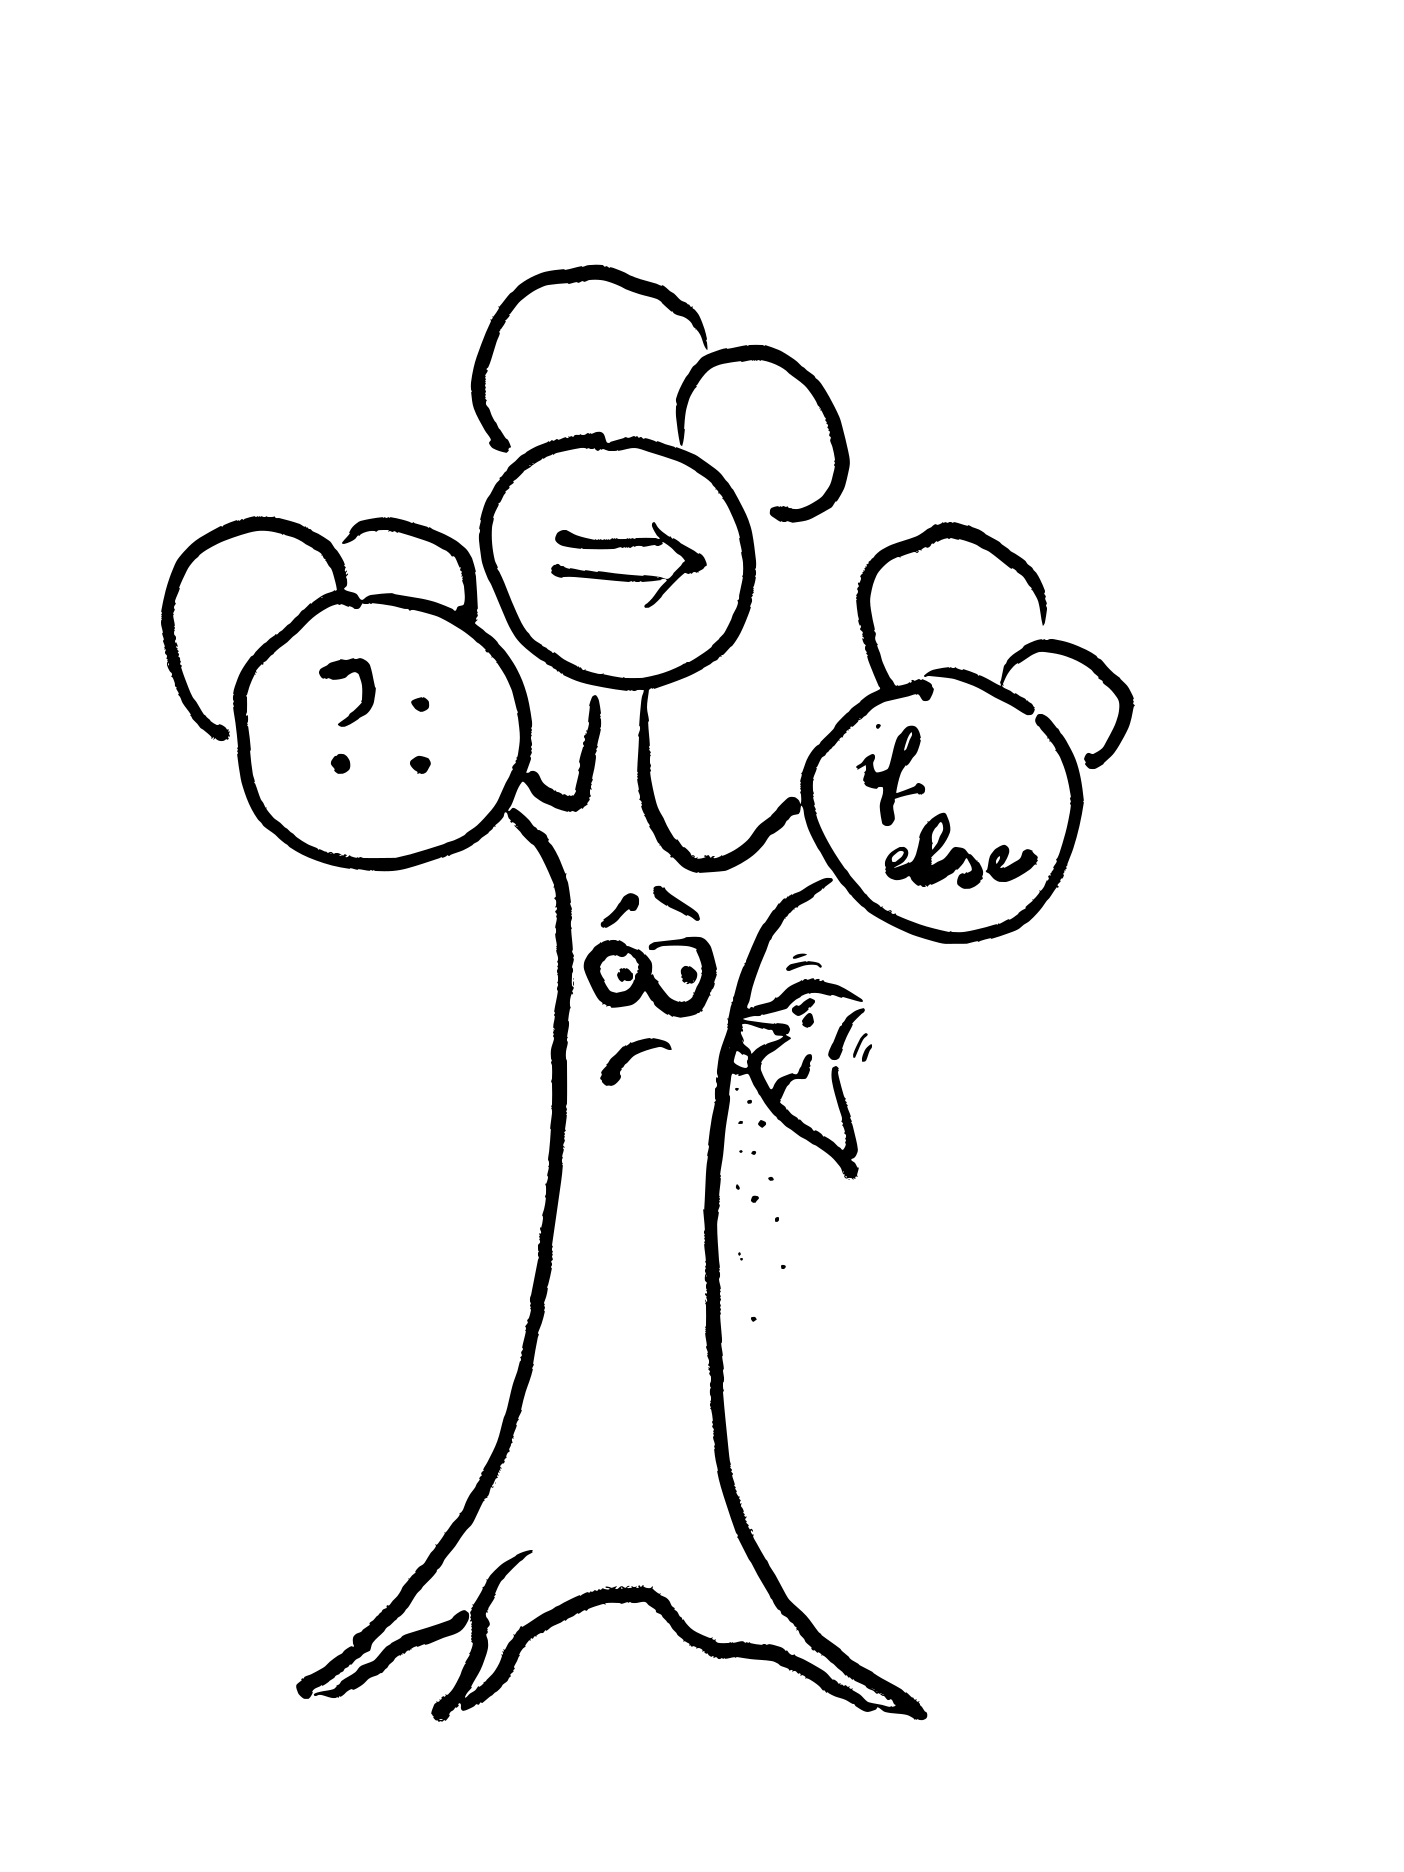
\includegraphics[width=0.9\textwidth]{tree}
    \end{center}
    \newpage

    \section{Approach}

    \subsection{Where to Join}

    \subsubsection{Conditional Expressions}

    Consider a conditional expression of the form $Ite(b, e_1, e_2)$.
    As Silicon evaluates this expression, and $b$ cannot definitely be evaluated to true or false,
    two branches are created, the first one assumes that $b$
    is true, and the second one that $b$ is false, and symbolic execution is continued for both branches.


    \subsubsection{Implications}

    Similar to conditional expressions, symbolic execution branches on implications too. Consider
    an implication of the form $b \implies i$. The first branch assumes that $b$ is true and
    consequently the implication $i$ holds. The second branch assumes that $b$ is false and the
    implication $i$ may or may not hold. 

    \subsubsection{If-Statements} \label{approach:if-statements}

    Viper is parsed into a Control Flow Graph (CFG) consisting of blocks containing
    statements, and edges which connect blocks. Edges can be unconditional or conditional,
    and can potentially form cycles whenever a back edge is connected to a loop head block.
    Symbolic execution branches whenever a block has more than one outgoing edges.

    To join again at the correct location within the CFG after branching,
    the join point for each corresponding branch point has to be identified.
    We introduce a recursive algorithm which maps each branch point to its corresponding join point,
    if it exists:

    \begin{enumerate}
        \item Initialize a queue of blocks to visit and a list of already visited blocks.
            Traverse the CFG in a breath-first way.
        \item \emph{Recursive Case.} If a block has two outgoing edges, it is a branch point.
            Call this procedure recursively, starting from this branch point.
        \item \emph{Base Case.} If a block is visited which already is included in the visited list,
            return this block as it is the join point corresponding to the branch point where this procedure was called.
    \end{enumerate}

    Special attention has to be paid to loops. If our algorithm follows a back edge before finding a join point,
    it may do the recursion again for the same branch point. To avoid this, all already visited loop head blocks
    are remembered for later recursive invocations. Already visited loop head blocks are not followed again.
    Whenever a join point exists for a branch point created via if-statement, we can now join again similar to
    conditional expressions or implications.

    Branches created by both conditional expressions and implications are already being joined if they are pure.
    Branches resulting from impure conditional expressions and implications,
    and from all if-statements however aren't joined again, meaning that
    all statements later down the verification path are evaluated twice. Both of these
    verification paths may branch again, eventually leading to exponential growth in branches.

    When 

    \subsection{Merging the Symbolic State} \label{approach:merging-the-symbolic-state}
    
    We define a symbolic state $\sigma$ of type $\Sigma := (\Gamma, \Pi, H)$. The entries
    defined as follows:

    \begin{itemize}
        \item A store $\gamma$ of type $\Gamma := Var \to V$ maps local variables to their symbolic values.
        \item A path condition stack $\pi$ of type $\Pi$ records all assumptions that have been made in the current verification path.
        \item A symbolic heap $h$ of type $H$ that records which locations are accessible and their respective symbolic values.
    \end{itemize}

    For the following subsections, assume that after the verification branched under the condition $c$ of type $Bool$,
    two symbolic states $\sigma_1 = (\gamma_1, \pi_1, h_1)$ under the branch condition $c = c_1$, and
    $\sigma_2 = (\gamma_2, \pi_2, h_2)$ under the branch condition $\overline{c} = c_2$ are to be merged,
    resulting in the new state $\sigma_3 = (\gamma_3, \pi_3, h_3)$.

    Note that this core idea could be extended to merge more than two states at once. In practice however,
    no more than two states are merged at once.

    \subsubsection{Merging the Store}

    For merging stores $\gamma_1$ and $\gamma_2$, we consider two cases:

    \begin{enumerate}
        \item For some local variable $x$, we have $x \mapsto v_1 \in \gamma_1$ and $x \mapsto v_2 \notin \gamma_2$.
            In this case, we can simply omit $x$ in the new store $\gamma_3$ as we can assume that $x$ won't
            be needed later down the verification path.
        \item For some local variable $x$, we have $x \mapsto v_1 \in \gamma_1$ and $x \mapsto v_2 \in \gamma_2$.
            In this case, we modify the heap chunk such that $x \mapsto Ite(c_1, v_1, v_2) \in \gamma_3$.
    \end{enumerate}

    \subsubsection{Merging the Store (Dep.)}

    For merging stores $\gamma_1$ and $\gamma_2$, we consider two cases:

    \begin{enumerate}
        \item For some local variable $x$, we have $x \mapsto v_1 \in \gamma_1$ and $x \mapsto v_2 \notin \gamma_2$.
            In this case, we can simply omit $x$ in the new store $\gamma_3$ as we can assume that $x$ won't
            be needed later down the verification path.
        \item For some local variable $x$, we have $x \mapsto v_1 \in \gamma_1$ and $x \mapsto v_2 \in \gamma_2$.
            In this case, we introduce a new symbolic value $t$ and set $x \mapsto t \in \gamma_3$. We restrict the
            value of $t$ by adding $c_1 \implies t = v_1$ and $c_2 \implies t = v_2$ to the path condition
            stack $\pi_1 = \pi_2$ resulting in $pi_3$.
    \end{enumerate}

    \subsubsection{Merging the Heap}

    A heap is essentially a collection of heap chunks, where each heap chunk provides information
    about the location's value and the receiver's permission amount to the location.
    As there may be multiple heap chunks making statements about aliased receivers,
    Silicon provides a mechanism to merge them using a mechanism called state consolidation.
    To merge heaps $h_1$ and $h_2$, we perform the following steps:

    \begin{enumerate}
        \item Every heap chunk $c$ for which $c \in h_1$ and $c \in h_2$ holds can be carried over to $h_3$
            without modifications.
        \item Heap chunks $c := x.f \mapsto t \perm p$ where $c \in h_1$ and $c \notin h_2$ are modified to
            have permissions only if $c_1$ holds: $c' := x.f \mapsto t \perm Ite(c_1, p, 0) \in h_3$
        \item Finally, $h_3$ can be consolidated to avoid multiple aliasing heap chunks.
    \end{enumerate}

    This method of only modifying the permission amount forks for both quantified and non-quantified heap chunks.

    \subsubsection{Merging the Heap (Dep.)}

    For merging non-quantified heap chunks, we consider two cases:

    \begin{enumerate}
        \item For some aliases $x$ and $y$, we have $x.f \mapsto v_1 \perm p_1 \in h_1$ and $y.f \mapsto v_2 \perm p_2 \notin h_2$.
            In this case, we introduce new symbolic values $t$ and $p$ of type $Perm$ and set $x.f \mapsto t \perm p \in h_3$.
            We restrict the values of $t$ and $p$ by adding $c_1 \implies t = v_1 \land p = p_1$
            to the path condition stack $\pi_1 = \pi_2$ resulting in $\pi_3$.
        \item For some aliases $x$ and $y$, we have $x.f \mapsto v_1 \perm p_1 \in h_1$ and $y.f \mapsto v_2 \perm p_2 \in h_2$.
            In this case, we introduce new symbolic values $t$ and $p$ of type $Perm$ and set $x.f \mapsto t \perm p \in h_3$.
            We restrict the values of $t$ and $p$ by adding $c_1 \implies t = v_1 \land p = p_1$ and $c_2 \implies t = v_2 \land p = p_2$
            to the path condition stack $\pi_1 = \pi_2$ resulting in $\pi_3$.
    \end{enumerate}

    Quantified heap chunks are of the shape $\forall x: c(x) \implies e(x).f \mapsto v(x) \perm p(x)$.
    In practice, they are rewritten as $\forall x: e(x).f \mapsto v(x) \perm p'(x)$, where $p'(x)$ may be defined as:

    \begin{math}
        p'(x) = \begin{cases}
            p(x) & \text{if } c(x) \text{ is true,} \\
            0 & \text{else}
        \end{cases}
    \end{math}

    Now using the second representation of quantified heap chunks, we again consider two cases similar to merging non-quantified
    heap chunks:

    \begin{enumerate}
        \item For some aliases $x$ and $y$, we have $x.f \mapsto v_1 \perm p_1 \in h_1$ and $y.f \mapsto v_2 \perm p_2 \notin h_2$.
            In this case, we introduce new symbolic values $t$ and $p$ of type $Perm$ and set $x.f \mapsto t \perm p \in h_3$.
            We restrict the values of $t$ and $p$ by adding $c_1 \implies t = v_1 \land p = p_1$
            to the path condition stack $\pi_1 = \pi_2$ resulting in $\pi_3$.
        \item For some aliases $x$ and $y$, we have $x.f \mapsto v_1 \perm p_1 \in h_1$ and $y.f \mapsto v_2 \perm p_2 \in h_2$.
            In this case, we introduce new symbolic values $t$ and $p$ of type $Perm$ and set $x.f \mapsto t \perm p \in h_3$.
            We restrict the values of $t$ and $p$ by adding $c_1 \implies t = v_1 \land p = p_1$ and $c_2 \implies t = v_2 \land p = p_2$
            to the path condition stack $\pi_1 = \pi_2$ resulting in $\pi_3$.
    \end{enumerate}

    \subsubsection{Merging the Path Conditions}

    For path conditions, the functionality for merging is already provided.
    This is done by putting the collected path conditions of each branch
    under an implication with the corresponding branch condition.

    \section{Implementation}

    \subsection{Implementing State Merges}

    Store and heap merges are implemented as according to \ref{approach:merging-the-symbolic-state}.
    Silicon's state however consists of some more fields that have to be merged with caution.

    \subsection{Finding Join Points}

    To find join points within the CFG, the algorithm described in \ref{approach:if-statements} is implemented.
    The algorithm produces a mapping from each branch point to the respective join point.

    The recursive following of CFG edges is modified to return as soon as the join point is reached, and the
    branches are joined again.

    \section{Evaluation}

    \subsection{Concluding Performance Evaluation}

    \begin{figure}[H]
        \includegraphics[width=\linewidth]{state-merges-vs-performance.png}
        \caption{
            Impact on the number of state merges on the performance,
            negative relative performance difference shows a speedup.
        }
        \label{fig:state-merges}
    \end{figure}

    \subsection{Complementary Benchmarks}

    \subsubsection{Caches}

    \subsubsection{More Complete Exhale}

    \newpage
    \printbibliography
    
\end{document}